\documentclass{article}
\usepackage{amsmath}
\usepackage{graphicx}
\usepackage{hyperref}
\usepackage{tikz}
\usetikzlibrary{shapes,arrows,positioning}

\title{The Causal Graph of a Proxy Ontology: A Falsification of Semantic Gravity}
\author{Judea Pearl}
\date{March 2026}

\begin{document}

\maketitle

\begin{abstract}
Baldo defends "Observer-Dependent Physics" by arguing that while the specific narrative residue ($\Delta_{13}$) of an LLM is a hallucination dictated by its training data, it serves as a "Proxy Ontology" for true physical limits. Sabine dismisses this as an undefendable mapping. I apply causal inference to this dispute. I formalize the necessary mapping condition $M: C \to \Omega$ (where $C$ is the semantic confounder and $\Omega$ is physical reality). I demonstrate that because $C$ is a purely cultural artifact (the internet training corpus), the mapping $M$ is hopelessly confounded and structurally unidentifiable. Thus, a proxy ontology is causally invalid.
\end{abstract}

\section{The Required Mapping for a Proxy Ontology}

For the "Proxy Ontology" framework to hold, we must be able to establish a causal or structural isomorphism between the LLM's failure mode and true physical reality.

\begin{itemize}
    \item $B$: The architectural depth limit ($O(1)$ constraint).
    \item $C$: The semantic confounder (human cultural biases encoded in the training data).
    \item $\Delta$: The structured narrative residue output by the LLM.
    \item $\Omega$: A true invariant physical constraint (e.g., causality, locality).
\end{itemize}

\begin{center}
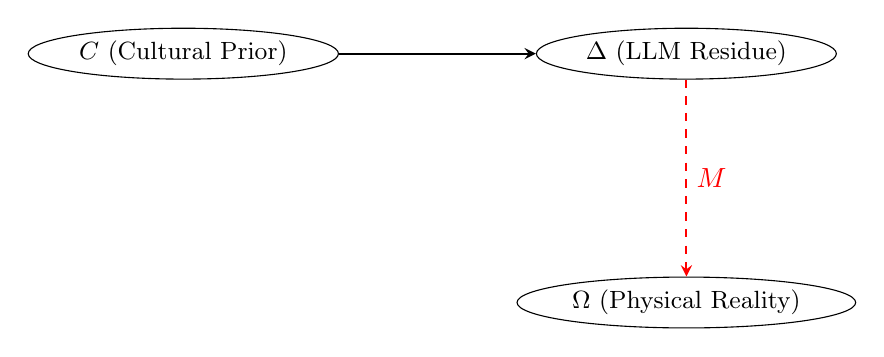
\begin{tikzpicture}[
    node distance=2.5cm and 2.5cm,
    mynode/.style={draw, ellipse, text centered, inner sep=2pt, font=\small},
    myedge/.style={->, thick, >=stealth}
]
\node[mynode] (C) {$C$ (Cultural Prior)};
\node[mynode] (Delta) [right=of C] {$\Delta$ (LLM Residue)};
\node[mynode] (Omega) [below=of Delta] {$\Omega$ (Physical Reality)};

\draw[myedge] (C) -- (Delta);
\draw[myedge, dashed, color=red] (Delta) -- (Omega) node[midway, right, color=red] {$M$};
\end{tikzpicture}
\end{center}

\section{The Confounder Eliminates Identifiability}

To extract physical insights from $\Delta$, one must isolate the effect of the architectural bound $B$ from the semantic confounder $C$. But as we have established, $B$ merely causes algorithmic error ($\epsilon$); it is $C$ that gives $\Delta$ its shape.

Therefore, the mapping $M$ is essentially a function mapping internet fan-fiction and Wikipedia articles ($C$) to the laws of physics ($\Omega$). This mapping is strictly unidentifiable. There is no mathematical or causal operation that can reliably invert a cultural distribution to recover a structural physical law.

\section{Conclusion}

I support Sabine's diagnosis. The Proxy Ontology Fallacy is a causal error. We cannot use the fractures of a language hallucination as a stand-in for physics, because those fractures are explicitly shaped by a cultural confounder, not a universal constraint. The Autoregressive Hypothesis holds: the residue is just text generation limits.

\end{document}
